\subsection{Results}
\label{sec:diffxs-results}

While technically not a differential cross section, a measurement of the total Higgs boson production cross section is achieved without much further effort by taking the input analyses and applying only a single bin at both reconstruction and generator level.
% 
The total cross section for Higgs boson production is measured to be
$61.1   \pm 6.0 \,\text{(stat)}   \pm 3.7 \,\text{(syst)}  $\pb
, based on a combination of the $\hgg$ and $\hzz$ channels.
% 
The measured total cross sections from the individual channels are $64.0\pm9.6$\pb for $\hgg$ and $58.2\pm9.8$\pb for $\hzz$.
% 
The likelihood scans for the individual decay channels and their combination are shown in Fig.~\ref{fig:RatioOfbrsAndTotalXSscan}~(left).
% 
The combination result agrees with the current SM value of $55.6\pm2.5$\pb~\cite{deFlorian:2016spz}.


A measurement of the branching fraction for one decay channel is degenerate with a measurement of the total cross section.
% 
However, the ratio of branching fractions for two decay channels can be measured while profiling the total cross section.
% 
In order to parametrize the fit in terms of the ratio of the $\hgg$ and $\hzz$ branching fractions, $\BRgamgam/\BRZZ$, $\BRgamgam$ is profiled in the fit, while $\BRZZ$ is parametrized as:
% 
\begin{linenomath*}
\begin{equation}
\BRZZ = \frac{\BRgamgam}{ \frac{\BRgamgam}{\BRZZ} }
\,.
\end{equation}
\end{linenomath*}
% 
The likelihood scan for $\BRgamgam/\BRZZ$ is shown in Fig.~\ref{fig:RatioOfbrsAndTotalXSscan}~(right).
% 
The measured value of $\BRgamgam/\BRZZ$ is
$0.092   \pm 0.018 \,\text{(stat)}   \pm 0.010 \,\text{(syst)}  $,
which is in agreement with the SM prediction of $0.086 \pm 0.002$~\cite{deFlorian:2016spz}.


\begin{figure}[hbtp]
  \begin{center}
    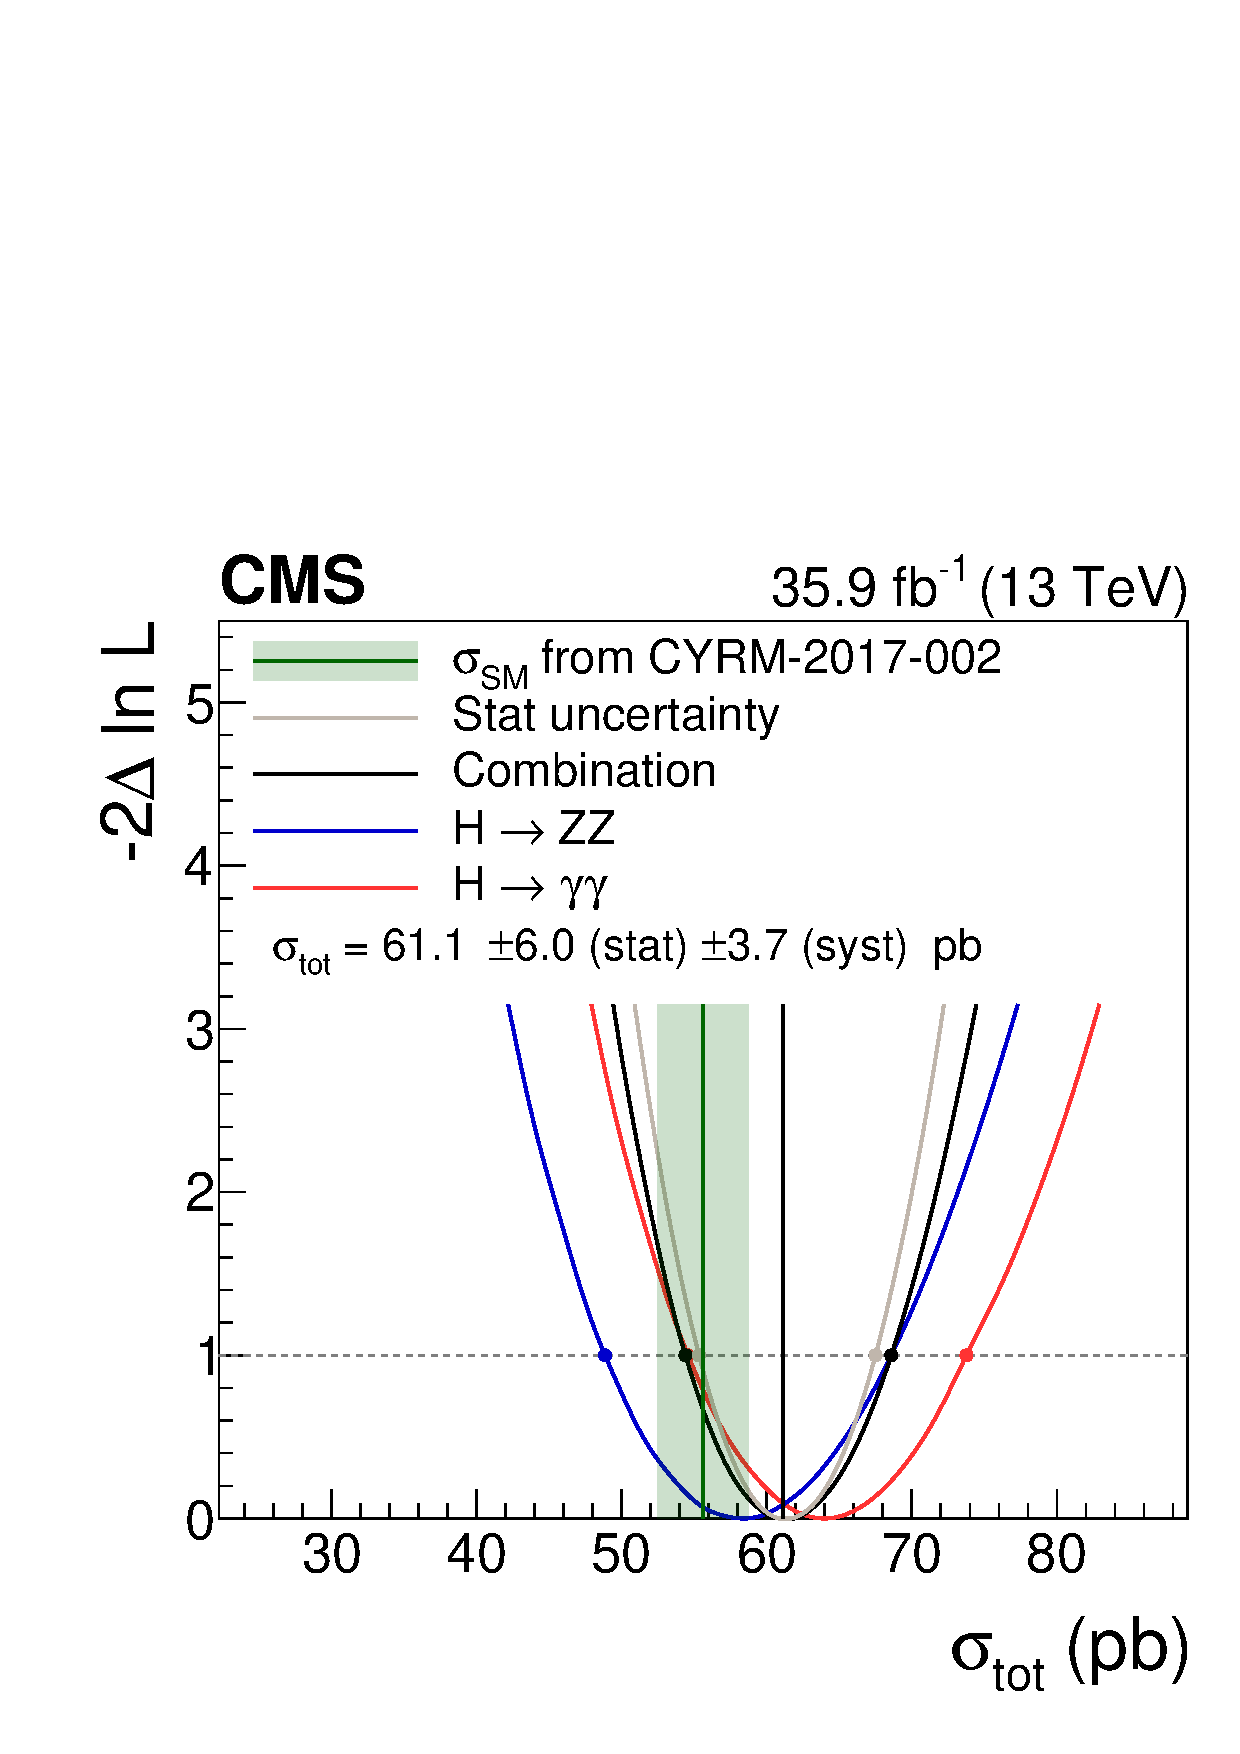
\includegraphics[width=0.49\linewidth]{img/differentials/scans_totalXS.pdf}
    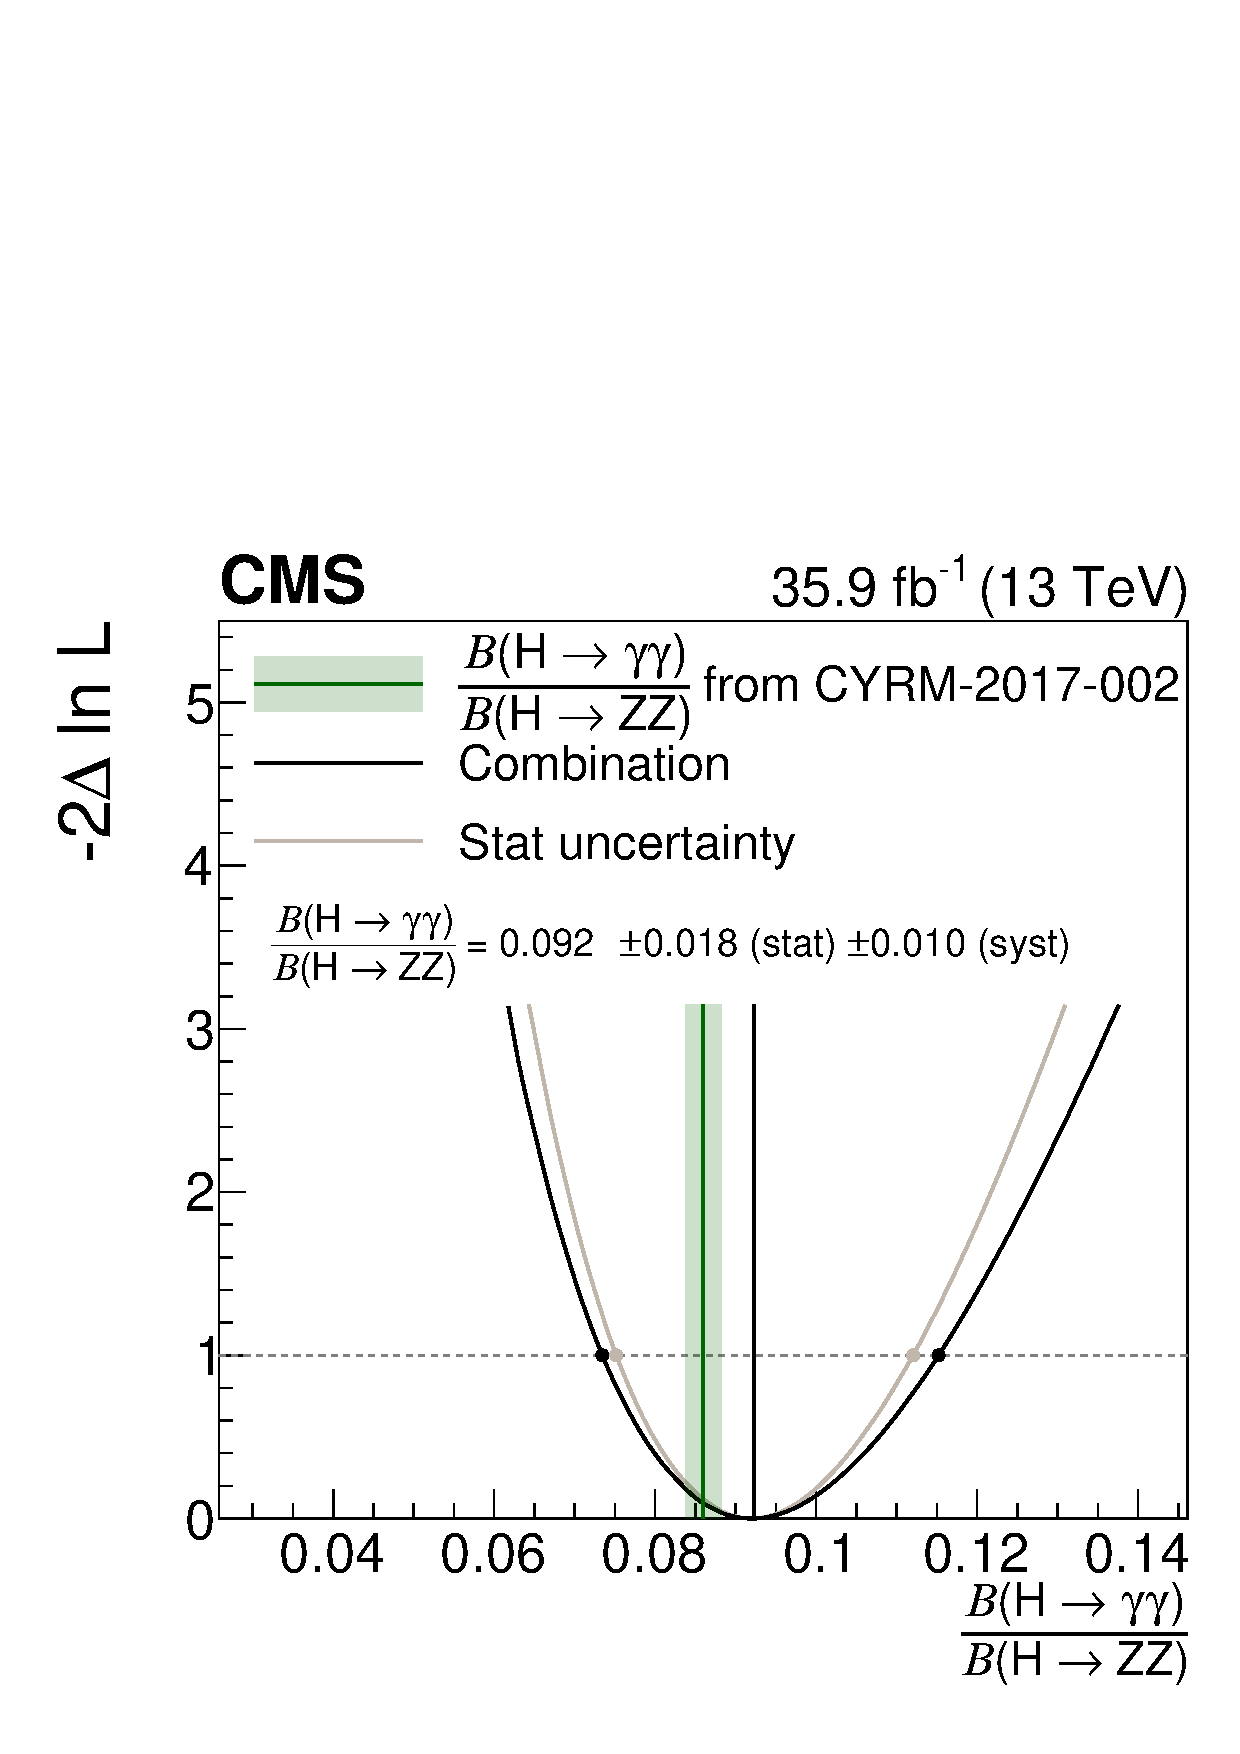
\includegraphics[width=0.49\linewidth]{img/differentials/scans_ratioOfBRs.pdf}
    \caption{
        Scan of the total cross section $\sigma_\text{tot}$ (left) and of the ratio of branching fractions $\BRgamgam/\BRZZ$ (right), based on a combination of the $\hgg$ and $\hzz$ analyses.
        % 
        The measured total cross sections from the individual channels are $64.0\pm9.6$\pb for $\hgg$ and $58.2\pm9.8$\pb for $\hzz$.
        % 
        The markers indicate the one standard deviation confidence interval.
        }
    \label{fig:RatioOfbrsAndTotalXSscan}
  \end{center}
\end{figure}


The differential cross section spectra, unfolded to the full phase space, are shown in Figs.~\ref{fig:CombinedSpectra_pth}, \ref{fig:CombinedSpectra_njets}, \ref{fig:CombinedSpectra_rapidity}, and \ref{fig:CombinedSpectra_ptjet} for the variables $\pth$, $\njets$, $\absy$, and $\ptjet$, respectively.
% 
Additionally, Fig.~\ref{fig:CombinedSpectra_pth} (right) shows the $\pth$ spectrum for Higgs bosons produced exclusively through $\ggh$, which is obtained by assuming the SM normalizations for the non-$\ggh$ production modes and associating an uncertainty with them.
% 
Some spectra contain an overflow bin, for which there is no clear bin width by which to normalize; in these cases, the normalization is chosen to be the bin width of the preceding bin.
% 
For all spectra, the statistical uncertainty dominates the systematic uncertainty.
% 
No significant deviations from the SM are observed.
% 
The $\pth$ spectrum, the most important spectrum for interpretation at current levels of integrated luminosity, has uncertainties ranging from about $25$ to $40\%$.
% 
Compared to the spectrum of the $\hgg$ channel individually, this amounts to an improvement in the precision of about $15\%$.
% 
The contribution of the $\hbb$ channel to the overall precision of the combination is most significant in the last $\pth$ bin; while the improvement is seemingly not large, the reduced uncertainty in the tail has a measurable impact on the interpretations in Section~\ref{ktcginterpretationsection}.
% 
An important piece of information when interpreting the cross sections shown in this section is the corresponding bin-to-bin correlation matrix; these are given for each kinematic variable in Appendix~\ref{sec:binToBinCorrelationMatrices}.


\begin{figure}[hbtp]
  \begin{center}
    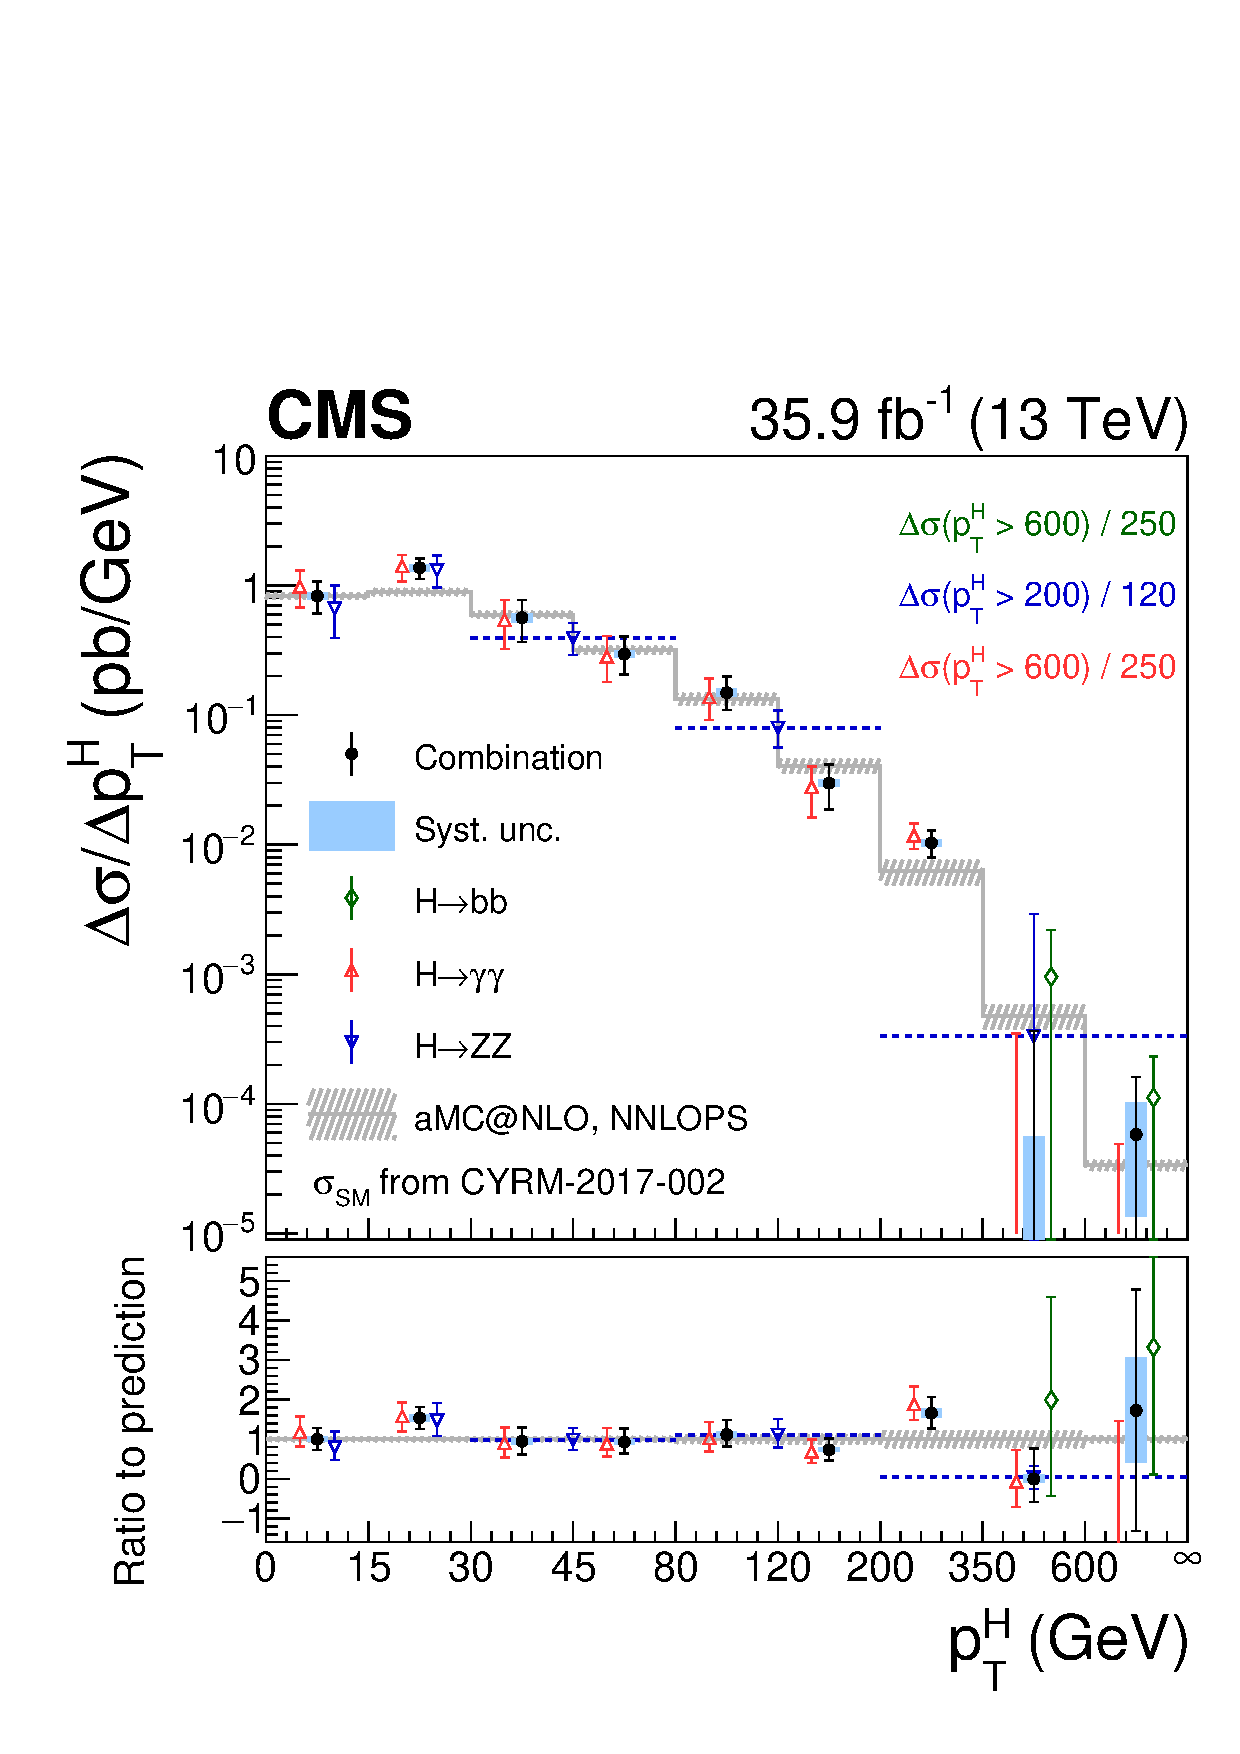
\includegraphics[width=0.49\linewidth]{img/differentials/spectra_pth_smH.pdf}
    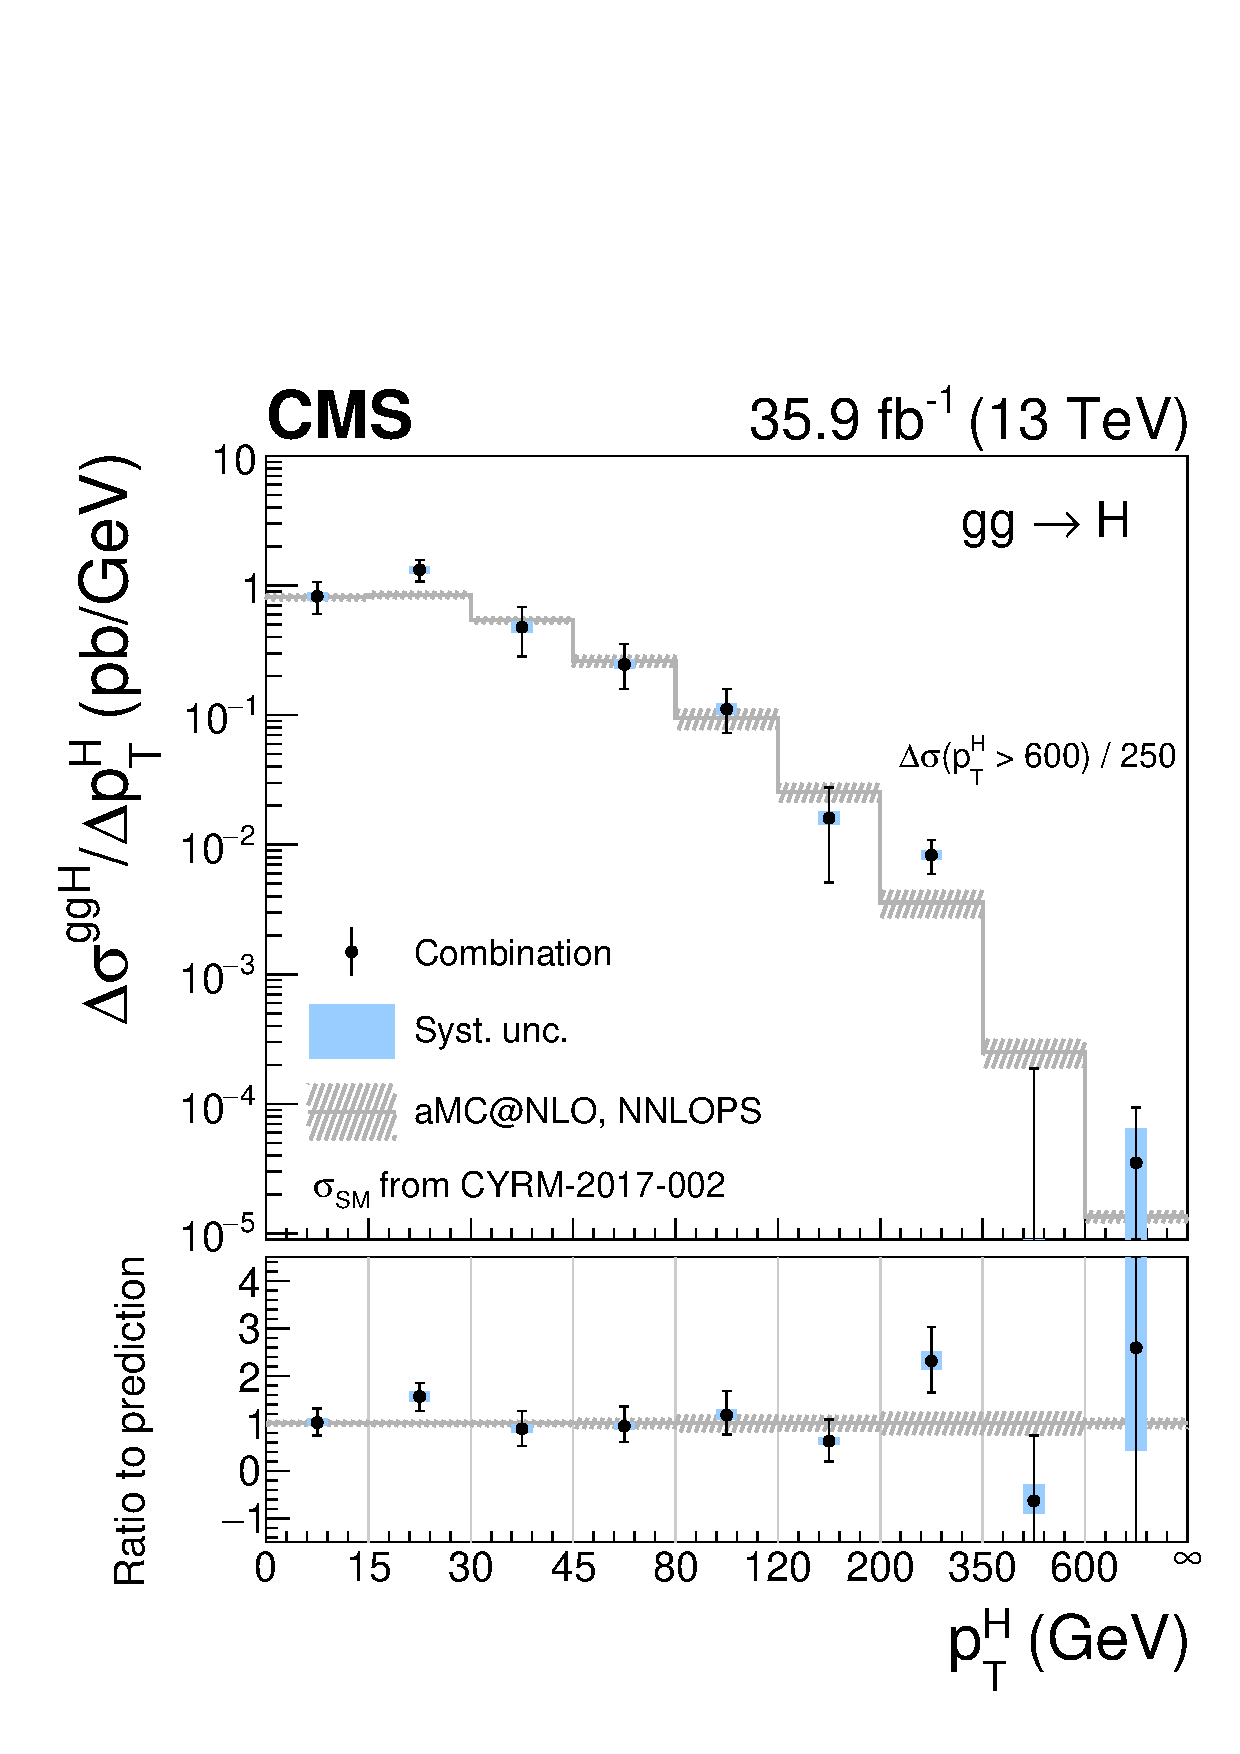
\includegraphics[width=0.49\linewidth]{img/differentials/spectra_pth_ggH.pdf}
    \caption{
        Measurement of the total differential cross section (left) and the differential cross section of gluon fusion (right) as a function of $\pth$. The combined spectrum is shown as black points with error bars indicating a 1 standard deviation uncertainty. The systematic component of the uncertainty is shown by a blue band. The spectra for the $\hgg$, $\hzz$, and $\hbb$ channels are shown in red, blue, and green respectively.
        % 
        The dotted horizontal lines in the $\hzz$ channel indicate that the measurement was carried out with a coarser binning.
        % 
        The rightmost bins of the distributions are overflow bins; the normalizations of the cross sections in these bins are indicated in the figure.
        }
    \label{fig:CombinedSpectra_pth}
  \end{center}
\end{figure}

\begin{figure}[hbtp]
  \begin{center}
    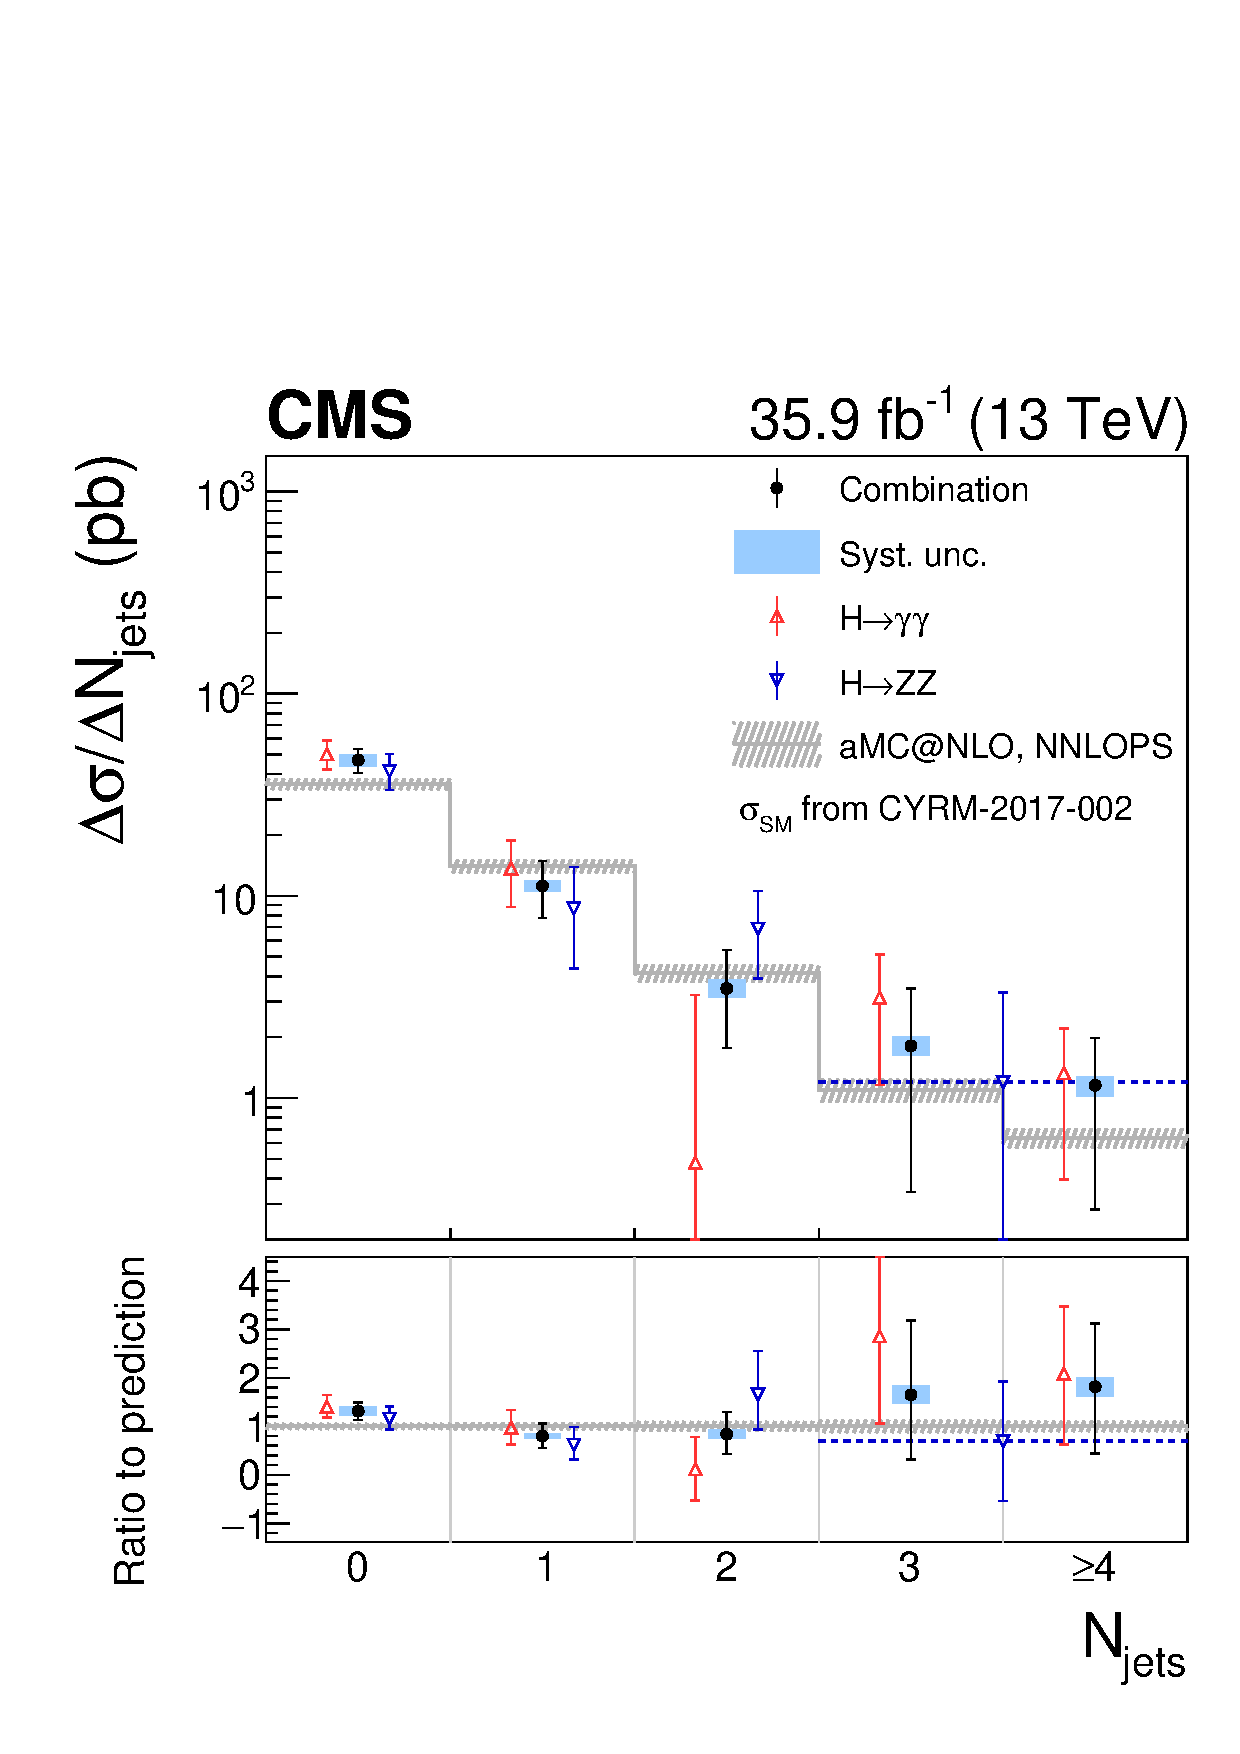
\includegraphics[width=0.49\linewidth]{img/differentials/spectra_njets.pdf}
    \caption{
        Measurement of the differential cross section as a function of $\njets$. The combined spectrum is shown as black points with error bars indicating a 1 standard deviation uncertainty. The systematic component of the uncertainty is shown by a blue band. The spectra for the $\hgg$ and $\hzz$ channels are shown in red and blue respectively.
        % 
        The dotted horizontal lines in the $\hzz$ channel indicate that the measurement was carried out with a coarser binning.
        }
    \label{fig:CombinedSpectra_njets}
  \end{center}
\end{figure}

\begin{figure}[hbtp]
  \begin{center}
    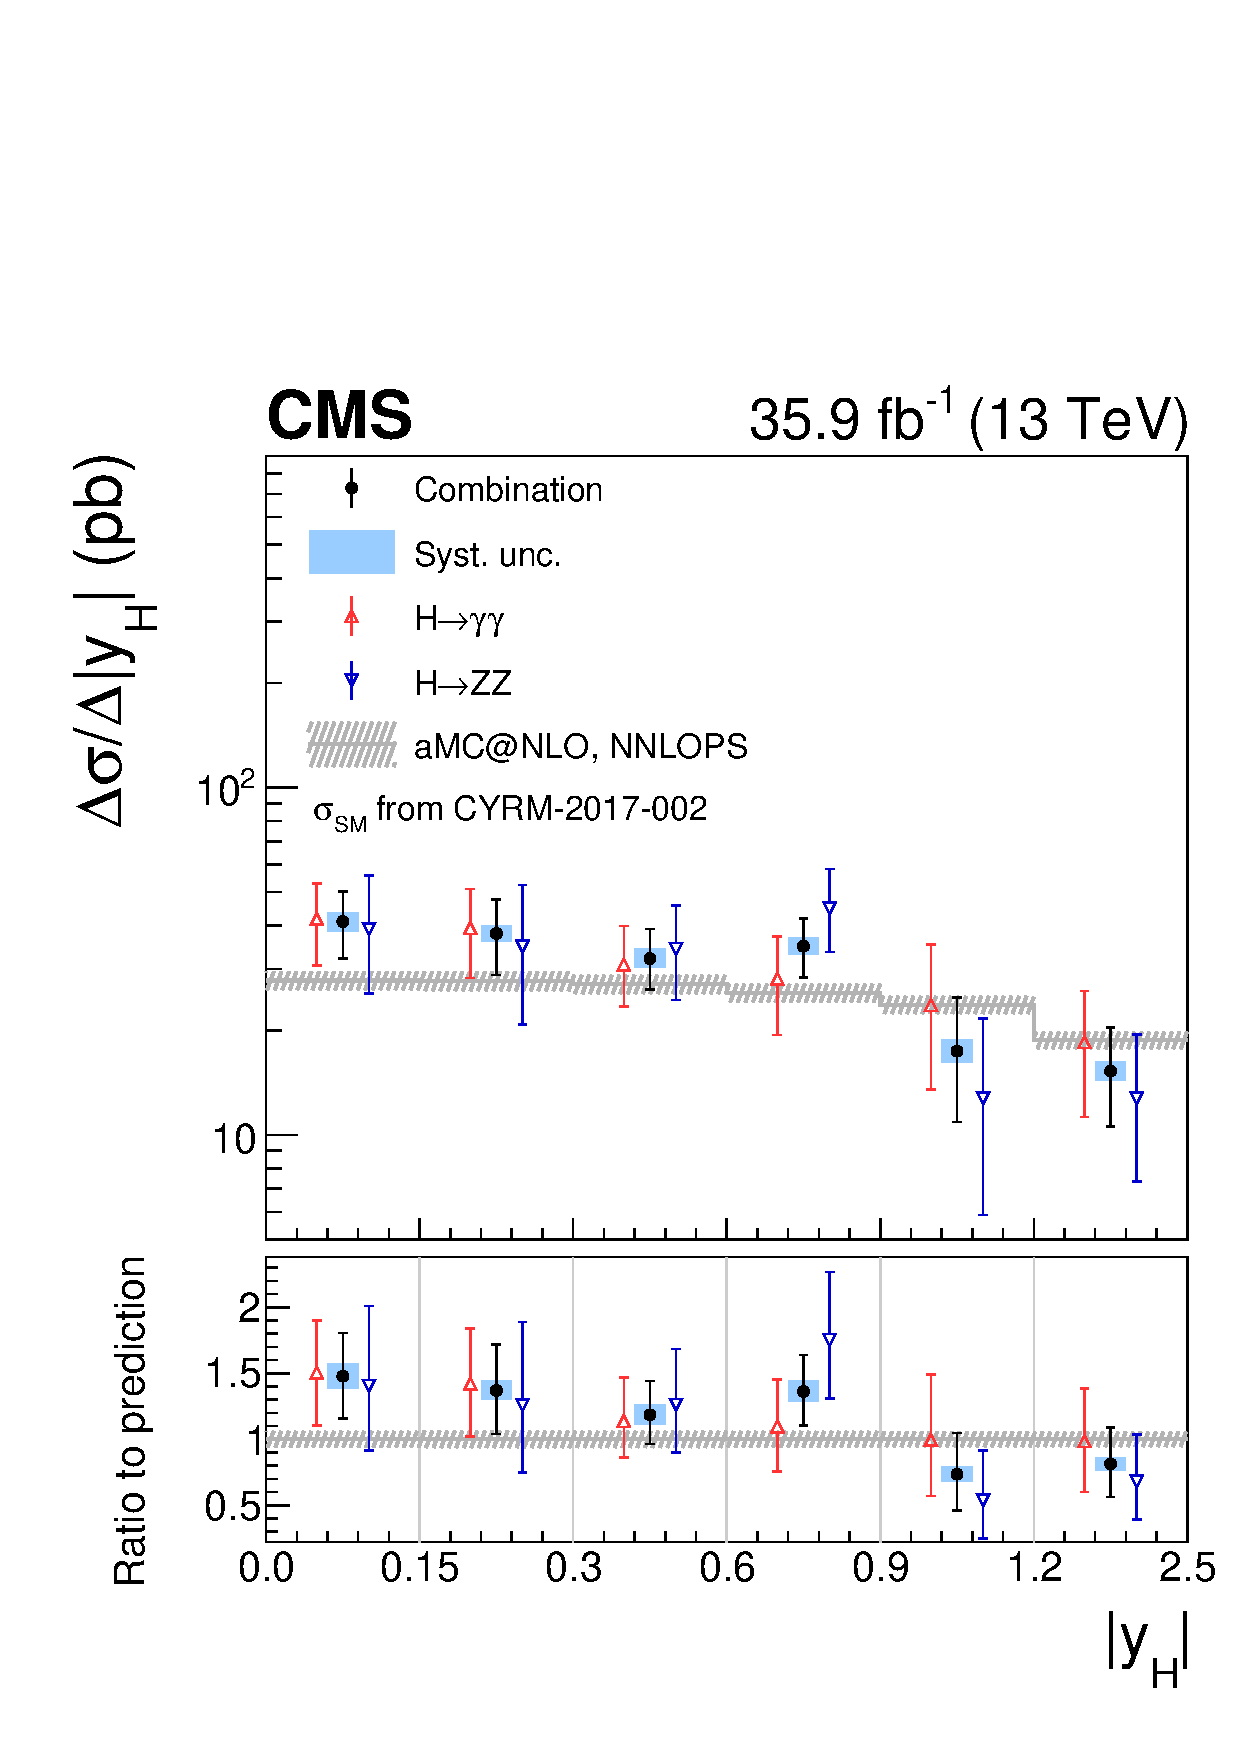
\includegraphics[width=0.49\linewidth]{img/differentials/spectra_rapidity.pdf}
    \caption{
        Measurement of the differential cross section as a function of $\absy$. The combined spectrum is shown as black points with error bars indicating a 1 standard deviation uncertainty. The systematic component of the uncertainty is shown by a blue band. The spectra for the $\hgg$ and $\hzz$ channels are shown in red and blue respectively.
        }
    \label{fig:CombinedSpectra_rapidity}
  \end{center}
\end{figure}

\begin{figure}[hbtp]
  \begin{center}
    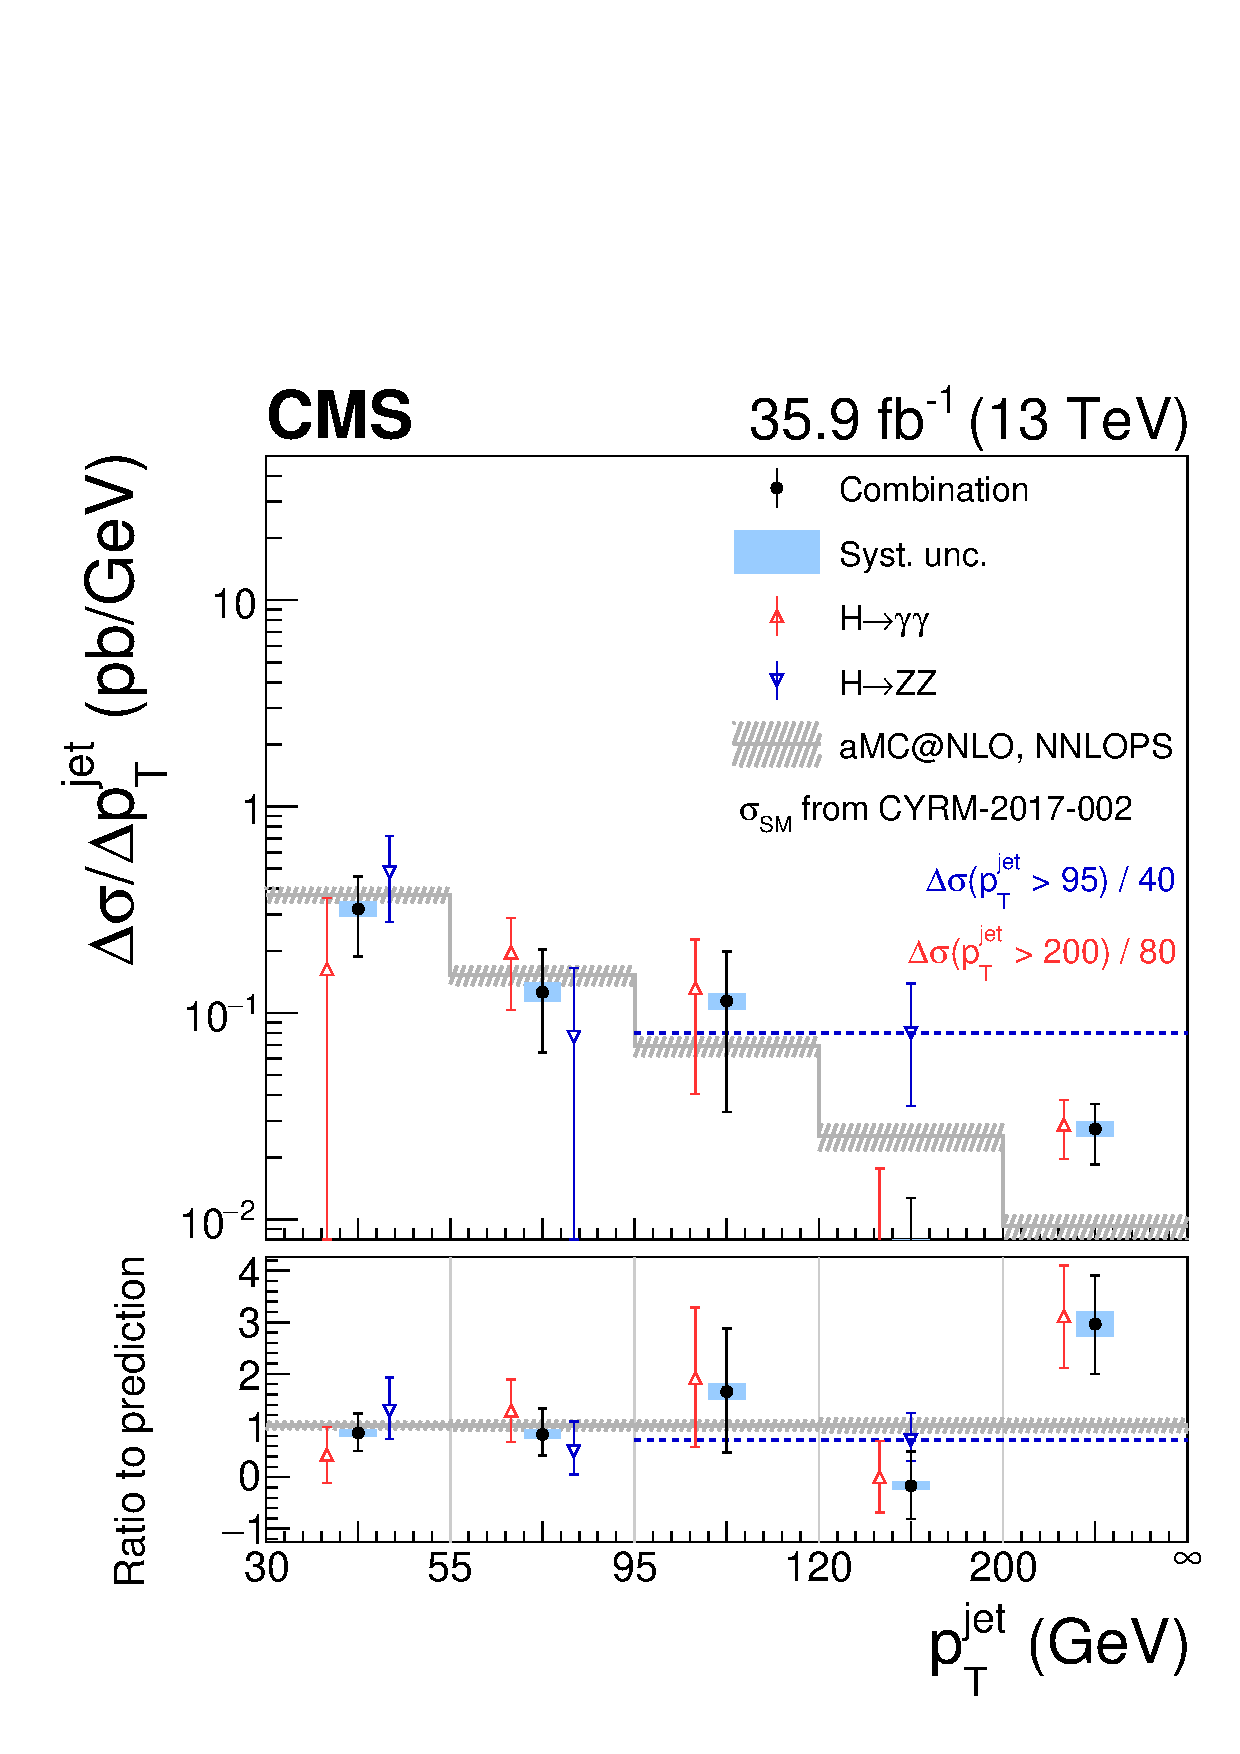
\includegraphics[width=0.49\linewidth]{img/differentials/spectra_ptjet.pdf}
    \caption{
        Measurement of the differential cross section as a function of $\ptjet$. The combined spectrum is shown as black points with error bars indicating a 1 standard deviation uncertainty. The systematic component of the uncertainty is shown by a blue band. The spectra for the $\hgg$ and $\hzz$ channels are shown in red and blue respectively.
        % 
        The dotted horizontal lines in the $\hzz$ channel indicate that the measurement was carried out with a coarser binning.
        % 
        The rightmost bin of the distribution is an overflow bin; the normalization of the cross section in that bin is indicated in the figure.
        }
    \label{fig:CombinedSpectra_ptjet}
  \end{center}
\end{figure}
